\documentclass{article}
\usepackage{amsmath}
\usepackage{amssymb}
\usepackage{graphicx}
\usepackage{hyperref}
\usepackage[version=4]{mhchem}

\title{Problem 10}
\date{}

\begin{document}
\maketitle

\section*{Problem}
\(A B C D\) is a trapezoid with \(A B / / D C . M\) and \(N\) are midpoints of \(A D\), \(B C\), respectively. \(M E / / D N\). \(M E\) meets \(A B\) at \(E\). Show that \(N E=D M\).\\
\centering
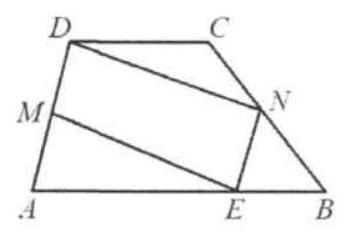
\includegraphics[width=\textwidth]{images/problem_image_1.jpg}

\section*{Solution}
Connect \(M N . M N\) is the median of the trapezoid \(A B C D\). So \(M N / / A B . \angle D M N=\) \(\angle M A E\).\\
Since \(M E / / D N, \angle M D N=\angle A M E\).\\
We also know that \(D M=M A\). Thus \(\triangle D M N \cong \triangle M A E\). So \(D N=M E\).\\
We also know that \(M E / / D N\). Therefore \(D N E M\) is a\\
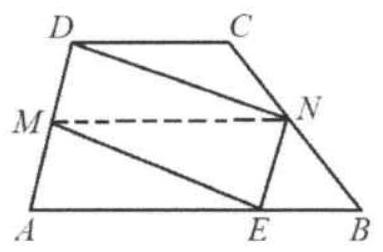
\includegraphics[width=\textwidth]{images/reasoning_image_1.jpg} parallelogram. Thus \(N E=D M\).

\end{document}
